\newpage
\section{Đặc tả yêu cầu bài toán}

\subsection{Giới thiệu chung}
Xác định các tác nhân của hệ thống
\noindent
\begin{table}[H]
    \centering
    \small % Duy trì cỡ chữ nhỏ để đồng bộ với các bảng khác
    \renewcommand{\arraystretch}{1.5} % Tạo khoảng cách dòng thông thoáng
    \setlength{\tabcolsep}{10pt} % Tăng khoảng cách lề cột để dễ quan sát
    
    \begin{tabularx}{\textwidth}{|c|>{\RaggedRight\arraybackslash\bfseries}p{4cm}|X|}
        \hline
        \rowcolor{gray!20} 
        \textbf{STT} & \textbf{Tên tác nhân} & \textbf{Mô tả tác nhân} \\ \hline
        
        1 & Người dùng & Người sử dụng ứng dụng. \\ \hline
        
        2 & Quản trị viên & Quản trị viên quản lý hệ thống. \\ \hline
    \end{tabularx}
    \caption{Bảng liệt kê và mô tả các tác nhân trong hệ thống}
    \label{tab:tac-nhan}
\end{table}
Xác định các ca sử dụng
\begin{table}[H]
    \centering
    \footnotesize % Sử dụng cỡ chữ nhỏ hơn để chứa được nhiều cột
    \renewcommand{\arraystretch}{1.5}
    \setlength{\tabcolsep}{3pt} % Tối ưu khoảng cách giữa các cột
    
    % Định nghĩa các cột: 
    % STT (c), Mã (c), Tên (p), Mô tả (X - tự giãn), Tác nhân (p), Độ phức tạp (c)
    \begin{tabularx}{\textwidth}{|c|c|>{\RaggedRight\arraybackslash}p{2.5cm}|X|>{\RaggedRight\arraybackslash}p{2.2cm}|c|}
        \hline
        \rowcolor{gray!20} 
        \textbf{STT} & \textbf{Mã UC} & \textbf{Tên Use Case} & \textbf{Mô tả Use Case} & \textbf{Tác nhân} & \textbf{Độ phức tạp} \\ \hline
        
        1 & UC001 & Quản lý danh sách mua sắm & Người dùng tạo, chỉnh sửa, xóa, theo dõi danh sách mặt hàng cần mua. Giao cho người dùng đi chợ. & Người dùng & Cao \\ \hline
        
        2 & UC002 & Quản lý dự định bữa ăn & Người dùng lên kế hoạch bữa ăn theo ngày hoặc tuần. & Người dùng & Cao \\ \hline
        
        3 & UC003 & Quản lý thực phẩm trong bếp & Người dùng nhập, chỉnh sửa, theo dõi thông tin thực phẩm tích trữ (tủ lạnh, bếp). & Người dùng & Thấp \\ \hline
        
        4 & UC004 & Quản lý công thức nấu ăn & Người dùng lưu trữ và quản lý các công thức nấu ăn. & Người dùng, Quản trị viên & Trung bình \\ \hline
        
        5 & UC005 & Quản lý danh sách thực phẩm & Người dùng quản lý danh sách các loại thực phẩm. & Người dùng, Quản trị viên & Trung bình \\ \hline
        
        6 & UC006 & Quản lý nhóm & Người dùng tạo/xóa nhóm, thêm/xóa thành viên trong nhóm. & Người dùng & Thấp \\ \hline
        
        7 & UC007 & Thống kê và báo cáo & Hệ thống tạo báo cáo về mua sắm và tiêu thụ thực phẩm. & Người dùng & Trung bình \\ \hline
        
        8 & UC008 & Quản trị người dùng & Quản trị viên quản lý tài khoản người dùng. & Quản trị viên & Thấp \\ \hline
    \end{tabularx}
    \caption{Bảng tổng hợp danh mục Use Case của hệ thống}
    \label{tab:danh-muc-usecase}
\end{table}
\subsection{Biểu đồ use case}
\subsubsection{Biểu đồ use case tổng quan}
\begin{figure}[H]
    \centering 
    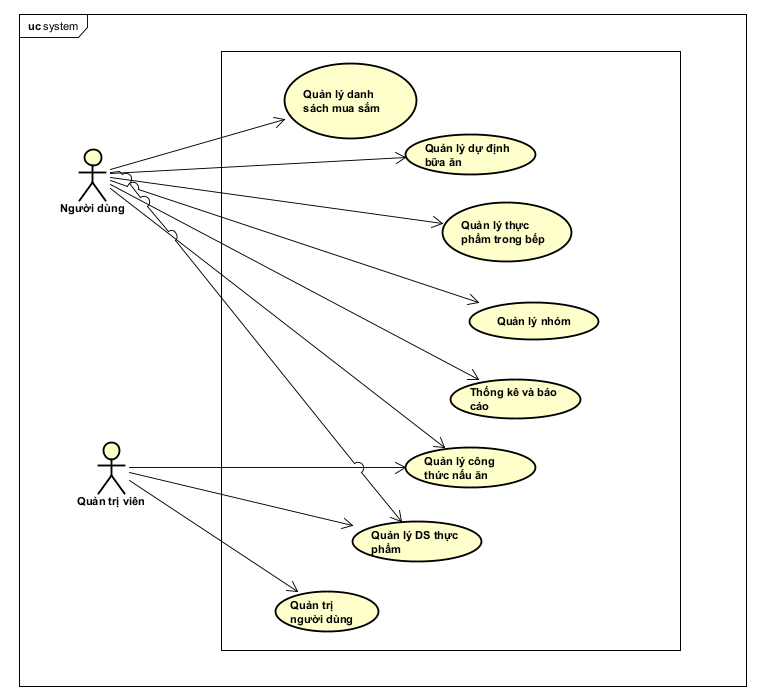
\includegraphics[width=0.9\textwidth]{UC_tong_quan.png}
    \caption{Biểu đồ Use Case tổng quan của hệ thống}
    \label{fig:usecase-tongquan}
\end{figure}
\subsubsection{Biểu đồ use case phân rã mức 2}
\textbf{Quản lý danh sách mua sắm}
\begin{figure}[H]
    \centering
    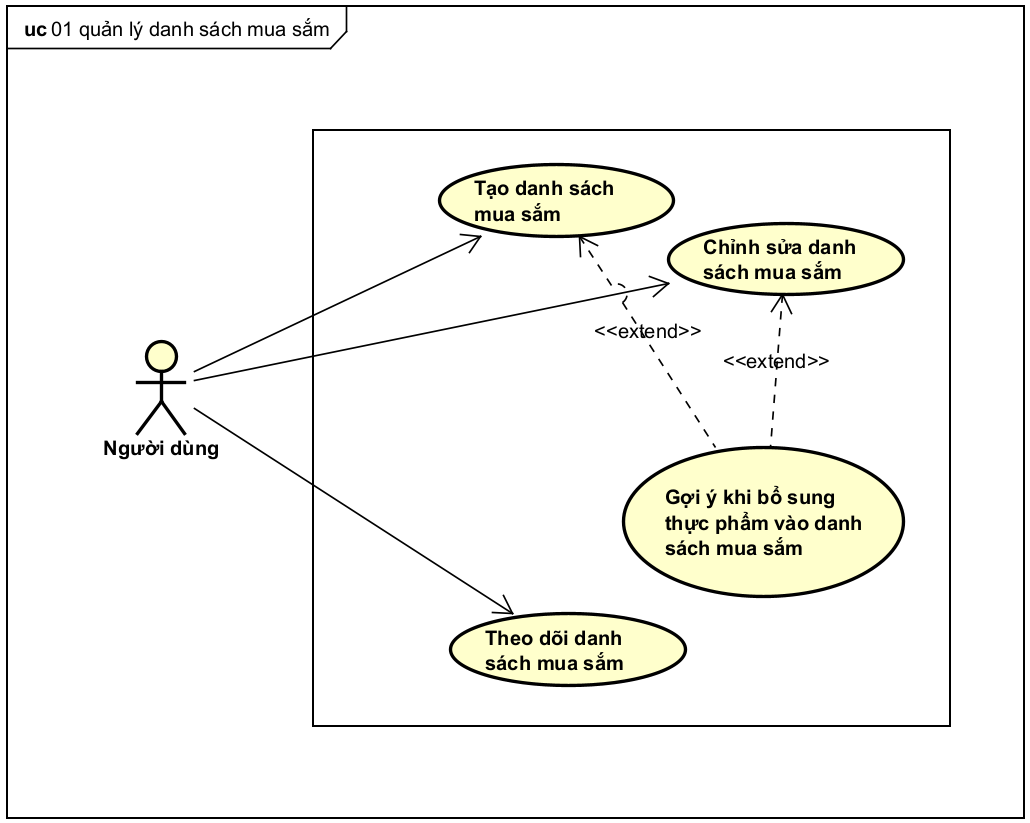
\includegraphics[width=0.9\textwidth]{UC_Danh_sach_mua_sam.png}
    \caption{Biểu đồ Usecase quản lý danh sách mua sắm}
    \label{fig:usecase-01}
\end{figure}

\vspace{1em}

\begin{table}[H]
    \centering
    \label{tab:uc001-1}
    \begin{tabularx}{\textwidth}{|c|p{3.5cm}|X|}
        \hline
        \rowcolor{headergreen} 
        \textbf{Mã UC} & \textbf{UC001.1} & \textbf{Tên UC: Tạo danh sách mua sắm} \\ \hline
        \textbf{Tác nhân} & \multicolumn{2}{l|}{Người dùng} \\ \hline
        \textbf{Điều kiện trước} & \multicolumn{2}{X|}{Người dùng đã tham gia vào một group} \\ \hline
        
        \multicolumn{3}{|c|}{\cellcolor{headerorange}\textbf{Luồng thực thi chính}} \\ \hline
        \rowcolor{graybg} \textbf{STT} & \textbf{Thực hiện} & \textbf{Hành động} \\ \hline
        1 & Người dùng & Điền thực phẩm cần mua \\ \hline
        2 & Người dùng & Chọn người đảm nhận \\ \hline
        3 & Người dùng & Hoàn thành tạo danh sách \\ \hline
        4 & Hệ thống & Lưu vào database \\ \hline
        5 & Hệ thống & Gửi thông báo cho người đảm nhận \\ \hline
        
        \multicolumn{3}{|c|}{\cellcolor{headerorange}\textbf{Luồng thực thi mở rộng}} \\ \hline
        \rowcolor{graybg} \textbf{STT} & \textbf{Thực hiện} & \textbf{Hành động và Điều kiện} \\ \hline
        1a & Hệ thống & \textbf{Điều kiện:} Trong group có thực đơn lên sẵn \newline \textbf{Hành động:} Thực hiện Usecase UC001.4 (Gợi ý bổ sung thực phẩm) \\ \hline
        
        \textbf{Điều kiện sau} & \multicolumn{2}{X|}{Danh sách mua sắm được tạo ra, người đảm nhiệm nhận được thông báo} \\ \hline
    \end{tabularx}
    \caption{Đặc tả ca sử dụng UC001.1: Tạo danh sách mua sắm}
\end{table}

\begin{table}[H]
    \centering
    \label{tab:uc001-3}
    \begin{tabularx}{\textwidth}{|c|p{3.5cm}|X|}
        \hline
        \rowcolor{headergreen} 
        \textbf{Mã UC} & \textbf{UC001.3} & \textbf{Tên UC: Theo dõi danh sách mua sắm} \\ \hline
        \textbf{Tác nhân} & \multicolumn{2}{l|}{Người dùng} \\ \hline
        \textbf{Điều kiện trước} & \multicolumn{2}{X|}{Group đã có danh sách mua sắm tạo trước đó} \\ \hline
        
        \multicolumn{3}{|c|}{\cellcolor{headerorange}\textbf{Luồng thực thi chính}} \\ \hline
        \rowcolor{graybg} \textbf{STT} & \textbf{Thực hiện} & \textbf{Hành động} \\ \hline
        1 & Người dùng & Mở danh sách mua sắm (hiển thị dưới dạng checklist). \\ \hline
        2 & Người dùng & Tick chọn một mặt hàng khi đã mua. \\ \hline
        3 & Hệ thống & Hiển thị hộp thoại nhập số lượng thực tế mua được. \\ \hline
        4 & Người dùng & Nhập số lượng thực tế và xác nhận. \\ \hline
        5 & Hệ thống & Ghi nhận số lượng thực tế đã mua: \newline
        - Nếu số lượng thực tế = số lượng dự định $\rightarrow$ đánh dấu ``đã mua''. \newline
        - Nếu số lượng thực tế < số lượng dự định $\rightarrow$ đánh dấu ``đã mua'' và tạo thêm 1 mục cần mua là số lượng thực phẩm đó còn thiếu. \\ \hline
        6 & Người dùng & Lặp lại cho các mặt hàng khác. \\ \hline
        7 & Người dùng & Chọn hoàn thành đi chợ. \\ \hline
        8 & Người dùng & Gửi thông báo đến toàn group. \\ \hline
        
        \textbf{Điều kiện sau} & \multicolumn{2}{X|}{Thông báo hoàn thành đi chợ được gửi đến toàn group} \\ \hline
    \end{tabularx}
    \caption{Đặc tả ca sử dụng UC001.3: Theo dõi danh sách mua sắm}
\end{table}

\begin{table}[H]
    \centering
    \label{tab:uc001-4}
    \begin{tabularx}{\textwidth}{|c|p{3.5cm}|X|}
        \hline
        \rowcolor{headergreen} 
        \textbf{Mã UC} & \textbf{UC001.4} & \textbf{Tên UC: Gợi ý bổ sung thực phẩm} \\ \hline
        \textbf{Tác nhân} & \multicolumn{2}{l|}{Người dùng} \\ \hline
        \textbf{Điều kiện trước} & \multicolumn{2}{X|}{Người dùng đang cần thêm một mục vào danh sách mua sắm; Trong group của người dùng có ``thực đơn lên sẵn''} \\ \hline
        
        \multicolumn{3}{|c|}{\cellcolor{headerorange}\textbf{Luồng thực thi chính}} \\ \hline
        \rowcolor{graybg} \textbf{STT} & \textbf{Thực hiện} & \textbf{Hành động} \\ \hline
        1 & Hệ thống & Kiểm tra dữ liệu: \newline
        - \textbf{Thực đơn đã lên lịch:} Kiểm tra thực đơn cho những bữa sắp tới. \newline
        - \textbf{Công thức nấu ăn:} Kiểm tra nguyên liệu cần dùng trong thực đơn đó. \newline
        - \textbf{Bếp:} Kiểm tra nguyên liệu đó có trong bếp không. \\ \hline
        2 & Hệ thống & Kiểm tra điều kiện xem nguyên liệu đó có số lượng ít hơn hay khác đơn vị so với công thức hay không. \\ \hline
        3 & Hệ thống & Gợi ý thực phẩm nên bổ sung. \\ \hline
        4 & Người dùng & Chọn đồng ý để thêm thực phẩm vào danh sách mua sắm. \\ \hline
        
        \multicolumn{3}{|c|}{\cellcolor{headerorange}\textbf{Luồng thực thi mở rộng}} \\ \hline
        \rowcolor{graybg} \textbf{STT} & \textbf{Thực hiện} & \textbf{Hành động và Điều kiện} \\ \hline
        2a & Hệ thống & \textbf{Điều kiện:} Nếu thực phẩm đó đã đủ hoặc thừa. \newline
        \textbf{Hành động:} Quay lại bước 1 để tìm nguyên liệu tiếp theo. \\ \hline
        4a & Hệ thống & \textbf{Điều kiện:} Người dùng không đồng ý thêm thực phẩm đó. \newline
        \textbf{Hành động:} Quay lại bước 1 để tìm nguyên liệu tiếp theo. \\ \hline
        
        \textbf{Điều kiện sau} & \multicolumn{2}{X|}{Thực phẩm cần mua được gợi ý cho người dùng} \\ \hline
    \end{tabularx}
    \caption{Đặc tả ca sử dụng UC001.4: Gợi ý khi bổ sung thực phẩm vào danh sách mua sắm}
\end{table}
\textbf{Quản lý dự định bữa ăn }
\begin{figure}[H]
    \centering
    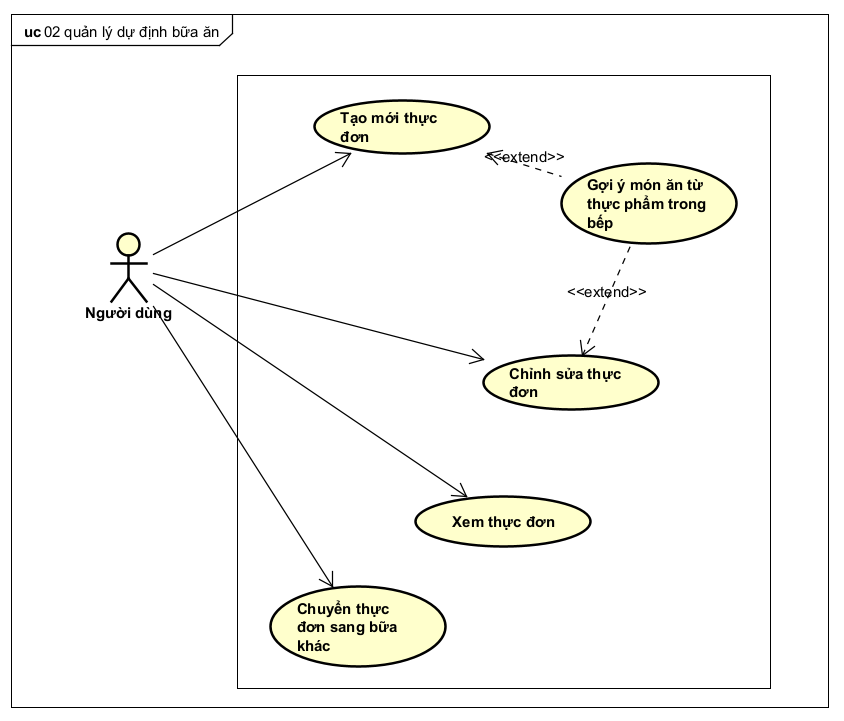
\includegraphics[width=0.9\textwidth]{UC_du_dinh_bua_an.png}
    \caption{Biểu đồ Usecase quản lý dự định bữa ăn}
    \label{fig:usecase-02}
\end{figure}
\begin{table}[H]
    \centering
    \label{tab:uc002-1}
    \begin{tabularx}{\textwidth}{|c|p{3.5cm}|X|}
        \hline
        \rowcolor{headergreen} 
        \textbf{Mã UC} & \textbf{UC002.1} & \textbf{Tên UC: Tạo thực đơn mới} \\ \hline
        \textbf{Tác nhân} & \multicolumn{2}{l|}{Người dùng} \\ \hline
        \textbf{Điều kiện trước} & \multicolumn{2}{X|}{Người dùng đã tham gia vào một group} \\ \hline
        
        \multicolumn{3}{|c|}{\cellcolor{headerorange}\textbf{Luồng thực thi chính}} \\ \hline
        \rowcolor{graybg} \textbf{STT} & \textbf{Thực hiện} & \textbf{Hành động} \\ \hline
        1 & Người dùng & Chọn bữa muốn tạo thực đơn. \\ \hline
        2 & Người dùng & Thêm từng món cho thực đơn. \\ \hline
        3 & Người dùng & Hoàn tất lên thực đơn. \\ \hline
        4 & Hệ thống & Lưu dữ liệu vào database. \\ \hline
        
        \multicolumn{3}{|c|}{\cellcolor{headerorange}\textbf{Luồng thực thi mở rộng}} \\ \hline
        \rowcolor{graybg} \textbf{STT} & \textbf{Thực hiện} & \textbf{Hành động và Điều kiện} \\ \hline
        2a & Hệ thống & \textbf{Điều kiện:} Nếu trong bếp có thực phẩm. \newline
        \textbf{Hành động:} Kích hoạt Usecase UC002.3. \\ \hline
        
        \textbf{Điều kiện sau} & \multicolumn{2}{X|}{Thực đơn mới được tạo ra} \\ \hline
    \end{tabularx}
    \caption{Đặc tả ca sử dụng UC002.1: Tạo thực đơn mới}
\end{table}
\begin{table}[H]
    \centering
    \label{tab:uc002-3}
    \begin{tabularx}{\textwidth}{|c|p{3.5cm}|X|}
        \hline
        \rowcolor{headergreen} 
        \textbf{Mã UC} & \textbf{UC002.3} & \textbf{Tên UC: Gợi ý món ăn từ thực phẩm trong bếp} \\ \hline
        \textbf{Tác nhân} & \multicolumn{2}{l|}{Người dùng} \\ \hline
        \textbf{Điều kiện trước} & \multicolumn{2}{X|}{Người dùng đang thêm món vào thực đơn, trong bếp đã có sẵn thực phẩm} \\ \hline
        
        \multicolumn{3}{|c|}{\cellcolor{headerorange}\textbf{Luồng thực thi chính}} \\ \hline
        \rowcolor{graybg} \textbf{STT} & \textbf{Thực hiện} & \textbf{Hành động} \\ \hline
        1 & Hệ thống & Kiểm tra: \newline
        - \textbf{Bếp:} Kiểm tra các thực phẩm có sẵn trong bếp. \newline
        - \textbf{Thực đơn:} Kiểm tra các món ăn sử dụng thực phẩm đó làm nguyên liệu chính. \\ \hline
        2 & Hệ thống & Gợi ý món ăn đó cho người dùng. \\ \hline
        3 & Người dùng & Đồng ý thêm món vào thực đơn. \\ \hline
        
        \multicolumn{3}{|c|}{\cellcolor{headerorange}\textbf{Luồng thực thi mở rộng}} \\ \hline
        \rowcolor{graybg} \textbf{STT} & \textbf{Thực hiện} & \textbf{Hành động và Điều kiện} \\ \hline
        2a & Hệ thống & \textbf{Điều kiện:} Chọn không đồng ý thêm món ăn. \newline
        \textbf{Hành động:} Quay lại bước 1 để gợi ý món ăn tiếp theo. \\ \hline
        
        \textbf{Điều kiện sau} & \multicolumn{2}{X|}{Thực đơn mới được tạo ra} \\ \hline
    \end{tabularx}
    \caption{Đặc tả ca sử dụng UC002.3: Gợi ý món ăn từ thực phẩm trong bếp}
\end{table}
\textbf{Quản lý thực phẩm trong bếp}
\begin{figure}[H]
    \centering 
    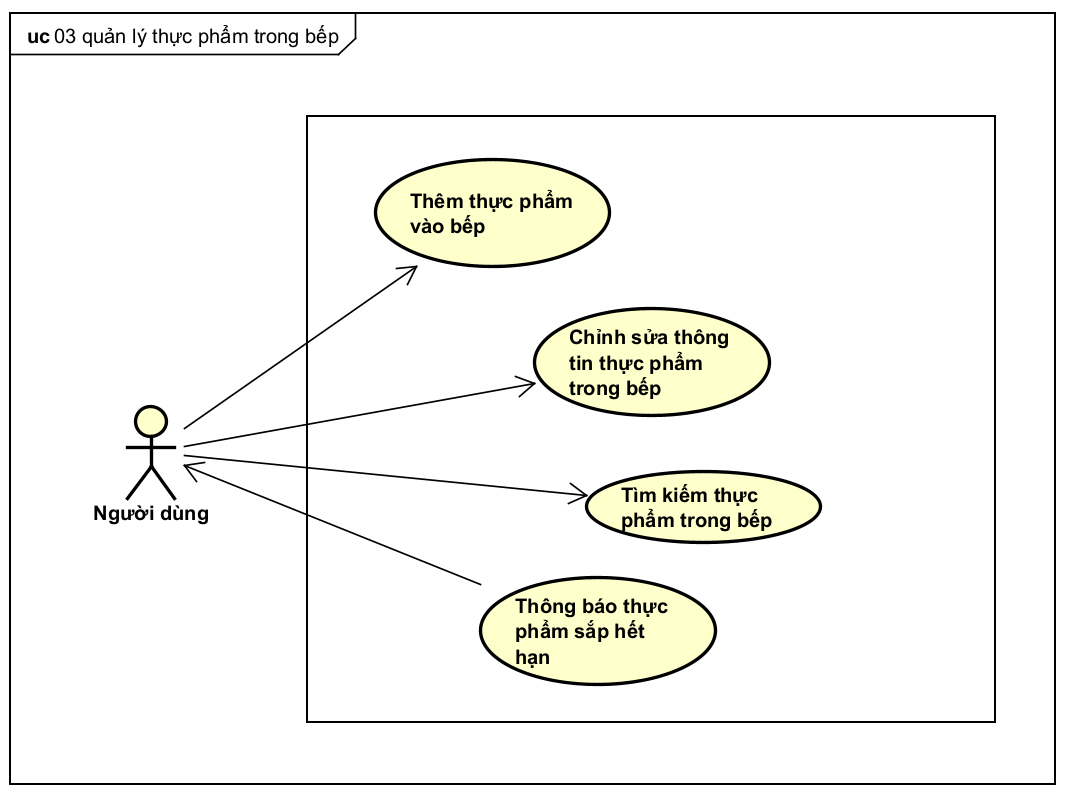
\includegraphics[width=0.9\textwidth]{UC_quan_ly_thucpham_trongbep.png}
    \caption{Biểu đồ Use Case quản lý thực phẩm trong bếp}
    \label{fig:usecase-03}
\end{figure}

\begin{table}[H]
    \centering
    \label{tab:uc003-1}
    \begin{tabularx}{\textwidth}{|c|p{3.5cm}|X|}
        \hline
        \rowcolor{headergreen} 
        \textbf{Mã UC} & \textbf{UC003.1} & \textbf{Tên UC: Thêm thực phẩm vào bếp} \\ \hline
        \textbf{Tác nhân} & \multicolumn{2}{l|}{Người dùng} \\ \hline
        \textbf{Điều kiện trước} & \multicolumn{2}{X|}{Người dùng đã tham gia vào một group} \\ \hline
        
        \multicolumn{3}{|c|}{\cellcolor{headerorange}\textbf{Luồng thực thi chính}} \\ \hline
        \rowcolor{graybg} \textbf{STT} & \textbf{Thực hiện} & \textbf{Hành động} \\ \hline
        1 & Người dùng & Chọn thêm thực phẩm. \\ \hline
        2 & Người dùng & Điền thông tin thực phẩm. \\ \hline
        3 & Hệ thống & Lưu dữ liệu vào database. \\ \hline
        
        \multicolumn{3}{|c|}{\cellcolor{headerorange}\textbf{Luồng thực thi mở rộng}} \\ \hline
        \rowcolor{graybg} \textbf{STT} & \textbf{Thực hiện} & \textbf{Hành động và Điều kiện} \\ \hline
        2a & Hệ thống & \textbf{Điều kiện:} Nếu trong bếp có thực phẩm. \newline
        \textbf{Hành động:} Kích hoạt Usecase UC002.3. \\ \hline
        
        \textbf{Điều kiện sau} & \multicolumn{2}{X|}{Thực phẩm mới được thêm vào trong bếp} \\ \hline
    \end{tabularx}
    \caption{Đặc tả ca sử dụng UC003.1: Thêm thực phẩm vào bếp}
\end{table}
\begin{table}[H]
    \centering
    \label{tab:uc003-2}
    \begin{tabularx}{\textwidth}{|c|p{3.5cm}|X|}
        \hline
        \rowcolor{headergreen} 
        \textbf{Mã UC} & \textbf{UC003.2} & \textbf{Tên UC: Chỉnh sửa thực phẩm trong bếp} \\ \hline
        \textbf{Tác nhân} & \multicolumn{2}{l|}{Người dùng} \\ \hline
        \textbf{Điều kiện trước} & \multicolumn{2}{X|}{Trong tủ lạnh đã có sẵn sản phẩm} \\ \hline
        
        \multicolumn{3}{|c|}{\cellcolor{headerorange}\textbf{Luồng thực thi chính}} \\ \hline
        \rowcolor{graybg} \textbf{STT} & \textbf{Thực hiện} & \textbf{Hành động} \\ \hline
        1 & Người dùng & Chọn thực phẩm cần chỉnh sửa. \\ \hline
        2 & Người dùng & Chỉnh sửa thông tin thực phẩm (Chỉ chỉnh sửa số lượng và đơn vị). \\ \hline
        3 & Hệ thống & Lưu dữ liệu vào database. \\ \hline
        
        \textbf{Điều kiện sau} & \multicolumn{2}{X|}{Thực phẩm được chỉnh sửa ở danh sách thực phẩm trong bếp} \\ \hline
    \end{tabularx}
    \caption{Đặc tả ca sử dụng UC003.2: Chỉnh sửa thực phẩm trong bếp}
\end{table}
\textbf{Quản lý công thức nấu ăn}
\begin{figure}[H]
    \centering 
    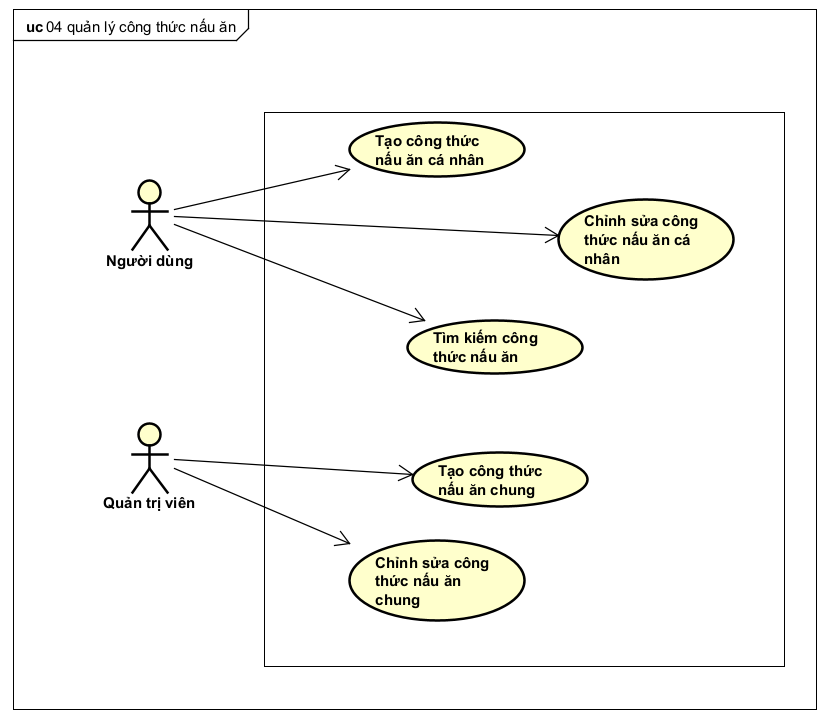
\includegraphics[width=0.9\textwidth]{UC_Quanly_congthuc.png}
    \caption{Biểu đồ Use Case quản lý công thức nấu ăn}
    \label{fig:usecase-04}
\end{figure}
\begin{table}[H]
    \centering
    \label{tab:uc004-1}
    \begin{tabularx}{\textwidth}{|c|p{3.5cm}|X|}
        \hline
        \rowcolor{headergreen} 
        \textbf{Mã UC} & \textbf{UC004.1} & \textbf{Tên UC: Tạo công thức nấu ăn chung} \\ \hline
        \textbf{Tác nhân} & \multicolumn{2}{l|}{Quản trị viên} \\ \hline
        \textbf{Điều kiện trước} & \multicolumn{2}{X|}{Quản trị viên đã đăng nhập} \\ \hline
        
        \multicolumn{3}{|c|}{\cellcolor{headerorange}\textbf{Luồng thực thi chính}} \\ \hline
        \rowcolor{graybg} \textbf{STT} & \textbf{Thực hiện} & \textbf{Hành động} \\ \hline
        1 & Quản trị viên & Chọn tạo công thức nấu ăn chung. \\ \hline
        2 & Quản trị viên & Điền thông tin cho công thức nấu ăn mới. \\ \hline
        3 & Quản trị viên & Hoàn thành điền thông tin. \\ \hline
        4 & Hệ thống & Lưu dữ liệu vào database. \\ \hline
        
        \textbf{Điều kiện sau} & \multicolumn{2}{X|}{Công thức nấu ăn chung mới được tạo ra} \\ \hline
    \end{tabularx}
    \caption{Đặc tả ca sử dụng UC004.1: Tạo công thức nấu ăn chung}
\end{table}
\begin{table}[H]
    \centering
    \label{tab:uc004-3}
    \begin{tabularx}{\textwidth}{|c|p{3.5cm}|X|}
        \hline
        \rowcolor{headergreen} 
        \textbf{Mã UC} & \textbf{UC004.3} & \textbf{Tên UC: Tạo công thức nấu ăn cá nhân} \\ \hline
        \textbf{Tác nhân} & \multicolumn{2}{l|}{Người dùng} \\ \hline
        \textbf{Điều kiện trước} & \multicolumn{2}{X|}{Người dùng đã tham gia vào nhóm} \\ \hline
        
        \multicolumn{3}{|c|}{\cellcolor{headerorange}\textbf{Luồng thực thi chính}} \\ \hline
        \rowcolor{graybg} \textbf{STT} & \textbf{Thực hiện} & \textbf{Hành động} \\ \hline
        1 & Người dùng & Chọn tạo công thức nấu ăn cho nhóm. \\ \hline
        2 & Người dùng & Điền thông tin cho công thức nấu ăn mới. \\ \hline
        3 & Người dùng & Hoàn thành điền thông tin. \\ \hline
        4 & Hệ thống & Lưu dữ liệu vào database. \\ \hline
        
        \textbf{Điều kiện sau} & \multicolumn{2}{X|}{Công thức nấu ăn cá nhân mới được tạo ra} \\ \hline
    \end{tabularx}
    \caption{Đặc tả ca sử dụng UC004.3: Tạo công thức nấu ăn cá nhân}
\end{table}
\begin{table}[H]
    \centering
    \label{tab:uc004-5}
    \begin{tabularx}{\textwidth}{|c|p{3.5cm}|X|}
        \hline
        \rowcolor{headergreen} 
        \textbf{Mã UC} & \textbf{UC004.5} & \textbf{Tên UC: Tìm kiếm công thức món ăn} \\ \hline
        \textbf{Tác nhân} & \multicolumn{2}{l|}{Người dùng} \\ \hline
        \textbf{Điều kiện trước} & \multicolumn{2}{X|}{Người dùng đã đăng nhập} \\ \hline
        
        \multicolumn{3}{|c|}{\cellcolor{headerorange}\textbf{Luồng thực thi chính}} \\ \hline
        \rowcolor{graybg} \textbf{STT} & \textbf{Thực hiện} & \textbf{Hành động} \\ \hline
        1 & Người dùng & Nhập vào thanh tìm kiếm tên món ăn hoặc nguyên liệu. \\ \hline
        2 & Hệ thống & Trả về danh sách món ăn. \\ \hline
        
        \textbf{Điều kiện sau} & \multicolumn{2}{X|}{Trả về danh sách kết quả các món ăn} \\ \hline
    \end{tabularx}
    \caption{Đặc tả ca sử dụng UC004.5: Tìm kiếm công thức món ăn}
\end{table}
\textbf{Quản lý danh sách thực phẩm}
\begin{figure}[H]
    \centering 
    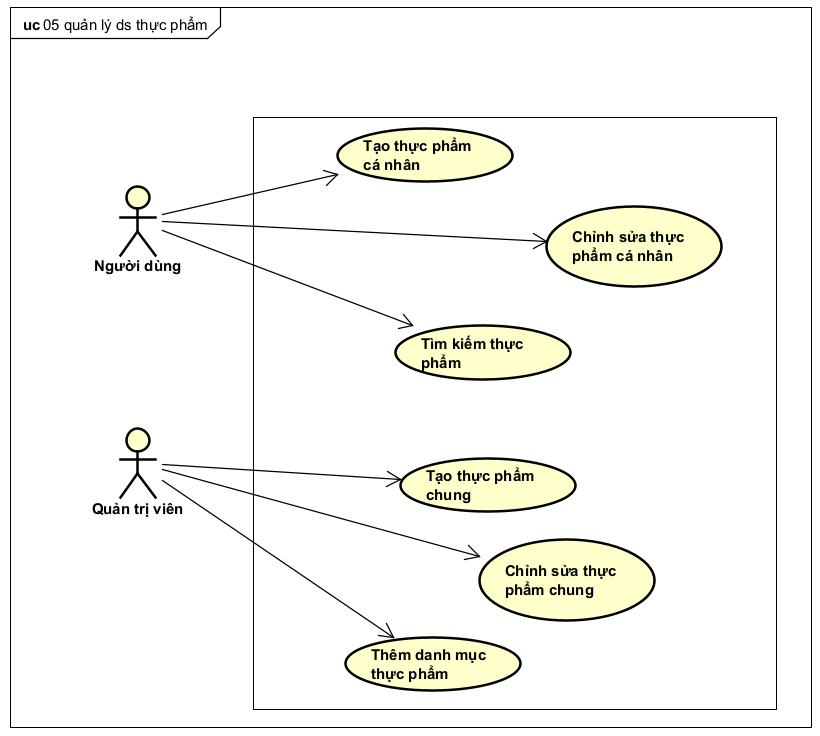
\includegraphics[width=0.9\textwidth]{UC_Quanly_danhsach_thucpham.png}
    \caption{Biểu đồ Use Case quản lý danh sách thực phẩm}
    \label{fig:usecase-05}
\end{figure}
\begin{table}[H]
    \centering
    \label{tab:uc005-1}
    \begin{tabularx}{\textwidth}{|c|p{3.5cm}|X|}
        \hline
        \rowcolor{headergreen} 
        \textbf{Mã UC} & \textbf{UC005.1} & \textbf{Tên UC: Tạo thực phẩm cá nhân} \\ \hline
        \textbf{Tác nhân} & \multicolumn{2}{l|}{Người dùng} \\ \hline
        \textbf{Điều kiện trước} & \multicolumn{2}{X|}{Người dùng đã tham gia vào nhóm} \\ \hline
        
        \multicolumn{3}{|c|}{\cellcolor{headerorange}\textbf{Luồng thực thi chính}} \\ \hline
        \rowcolor{graybg} \textbf{STT} & \textbf{Thực hiện} & \textbf{Hành động} \\ \hline
        1 & Người dùng & Chọn thực phẩm mới cho nhóm. \\ \hline
        2 & Người dùng & Điền thông tin cho thực phẩm mới. \\ \hline
        3 & Hệ thống & Kiểm tra tên thực phẩm có trùng không. \\ \hline
        4 & Người dùng & Hoàn thành tạo thực phẩm mới. \\ \hline
        5 & Hệ thống & Lưu dữ liệu vào database. \\ \hline
        
        \textbf{Điều kiện sau} & \multicolumn{2}{X|}{Thực phẩm cá nhân mới được tạo ra} \\ \hline
    \end{tabularx}
    \caption{Đặc tả ca sử dụng UC005.1: Tạo thực phẩm cá nhân}
\end{table}
\textbf{Quản lý nhóm}
\begin{figure}[H]
    \centering 
    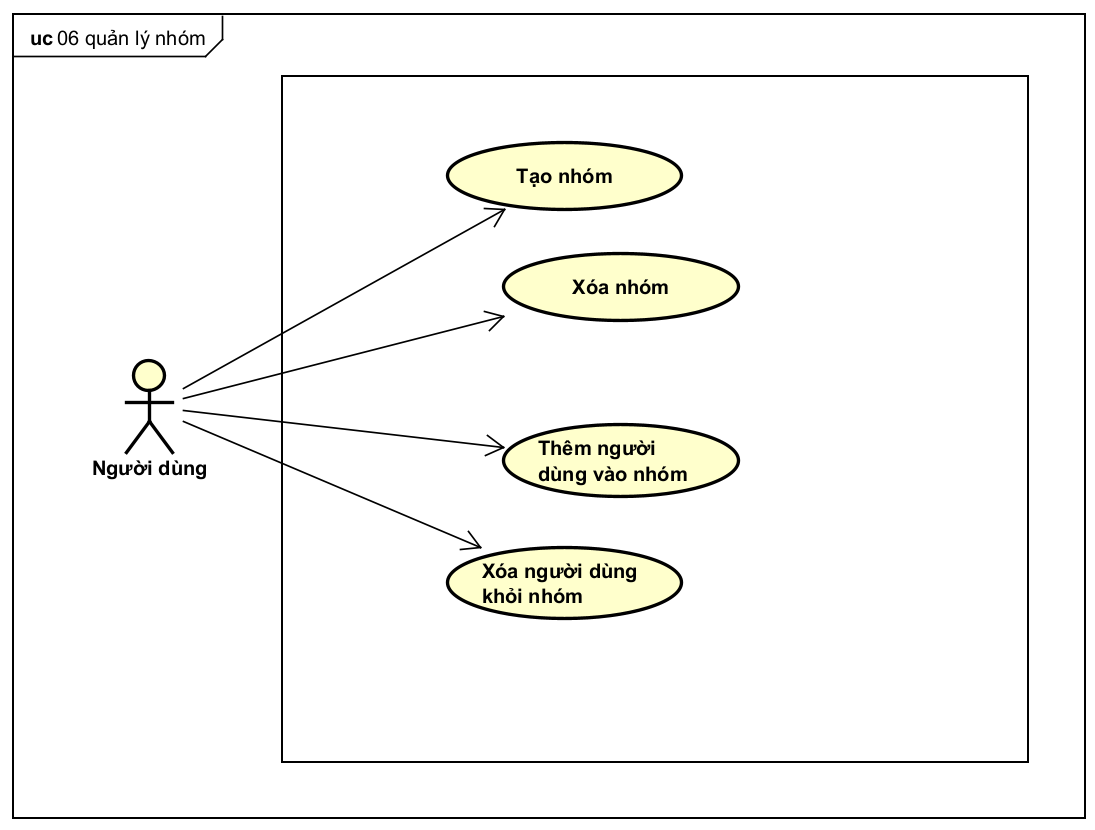
\includegraphics[width=0.9\textwidth]{UC_quanly_nhom.png}
    \caption{Biểu đồ Use Case quản lý nhóm}
    \label{fig:usecase-06}
\end{figure}
\textbf{Quản trị người dùng}
\begin{figure}[H]
    \centering 
    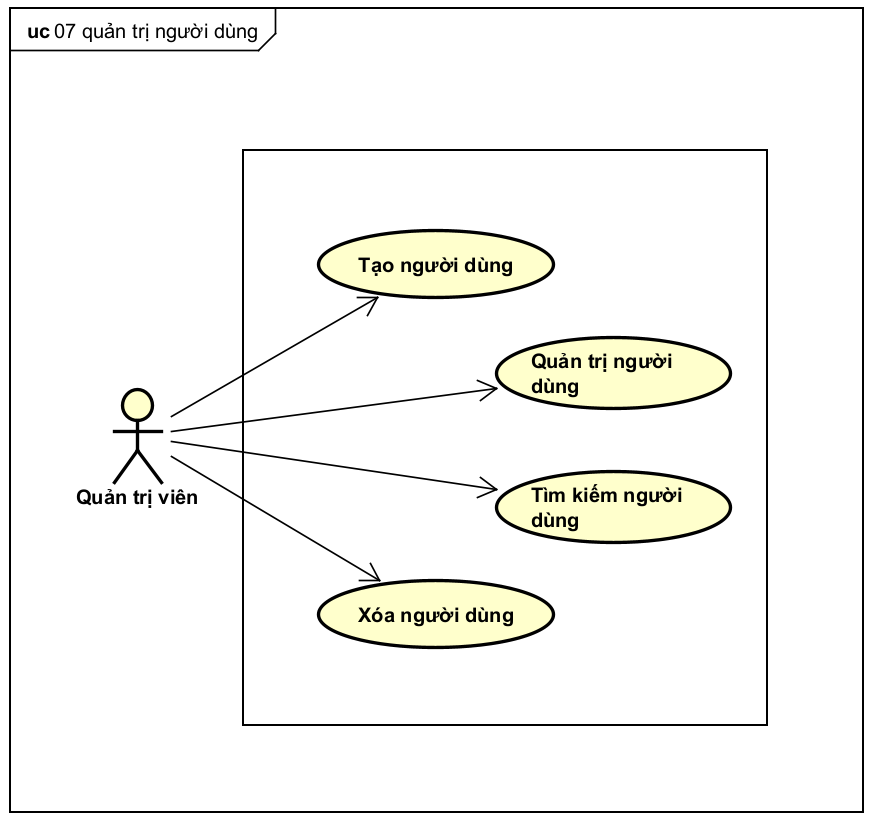
\includegraphics[width=0.9\textwidth]{UC_quanly_nguoidung.png}
    \caption{Biểu đồ Use Case quản lý người dùng}
    \label{fig:usecase-07}
\end{figure}
\subsection{Các yêu cầu phi chức năng}
\subsubsection{Tính dễ dùng}
\begin{itemize}
    \item Giao diện người dùng được thiết kế thân thiện, dễ hiểu, sử dụng được cho cả người dùng ít kinh nghiệm với công nghệ.
    \item Các thao tác như tạo, chỉnh sửa, xóa dữ liệu cần rõ ràng và có xác nhận trước khi thực hiện.
    \item Khi người dùng nhập sai dữ liệu, hệ thống phải hiển thị thông báo lỗi cụ thể, dễ hiểu, gồm:
    \begin{itemize}
        \item Mô tả lỗi (``Ngày hết hạn không hợp lệ'').
        \item Gợi ý cách khắc phục (``Vui lòng nhập ngày hợp lệ theo định dạng DD/MM/YYYY'').
    \end{itemize}
    \item Các biểu tượng và nút bấm có chú thích, gợi ý (tooltip, placeholder).
    \item Màu sắc, kích thước chữ, bố cục cần đảm bảo tính dễ đọc và nhất quán trên nhiều thiết bị (điện thoại, máy tính bảng).
\end{itemize}

\subsubsection{Hiệu năng}
\begin{itemize}
    \item Ứng dụng cần phản hồi các thao tác người dùng trong vòng 2 giây cho các chức năng cơ bản (tạo, sửa, xem danh sách, tìm kiếm).
    \item Tốc độ tải dữ liệu từ server phải đảm bảo mượt mà, không gây giật lag trong quá trình sử dụng.
    \item Cơ chế cache cục bộ được sử dụng để truy cập nhanh dữ liệu gần nhất khi thiết bị mất kết nối Internet.
    \item Hệ thống backend (server và CSDL) cần hỗ trợ tối thiểu 1000 người dùng đồng thời trong giai đoạn triển khai thử nghiệm.
\end{itemize}

\subsubsection{Tính tin cậy}
\begin{itemize}
    \item Hệ thống phải lưu trữ dữ liệu an toàn, không bị mất khi người dùng tắt ứng dụng đột ngột hoặc mất mạng.
    \item Dữ liệu người dùng được đồng bộ lên server ngay khi có kết nối mạng trở lại.
    \item Cơ chế sao lưu (backup) dữ liệu định kỳ mỗi ngày.
    \item Tự động phục hồi (auto-reconnect) khi mất kết nối ngắn hạn.
\end{itemize}

\subsubsection{Tính dễ bảo trì}
\begin{itemize}
    \item Mã nguồn được chia thành các module rõ ràng: frontend (giao diện), backend (API, xử lý logic), database (lưu trữ).
    \item Có tài liệu hướng dẫn cài đặt, cấu hình, và hướng dẫn lập trình viên mở rộng chức năng.
    \item Hệ thống được phát triển theo mô hình RESTful API, dễ dàng thay đổi hoặc mở rộng sang các nền tảng khác (web, desktop).
    \item Sử dụng công nghệ phổ biến, mã nguồn mở để dễ dàng bảo trì, cập nhật phiên bản.
\end{itemize}

\subsubsection{Tính khả chuyển}
\begin{itemize}
    \item Ứng dụng được phát triển bằng công nghệ đa nền tảng (ví dụ: Flutter hoặc React Native), có thể chạy trên cả Android và iOS.
    \item Cấu hình hệ thống linh hoạt, dễ dàng triển khai trên nhiều môi trường (local, cloud).
    \item Dữ liệu được lưu trữ trên cơ sở dữ liệu đám mây (ví dụ: Firebase, MongoDB Atlas hoặc MySQL Cloud).
\end{itemize}

\subsubsection{Yêu cầu an toàn bảo mật}
\begin{itemize}
    \item Dữ liệu người dùng được mã hóa khi truyền giữa client và server (sử dụng HTTPS).
    \item Mật khẩu người dùng phải được lưu trữ dưới dạng mã hóa (hash + salt).
    \item Mỗi tài khoản người dùng chỉ được phép truy cập và chỉnh sửa dữ liệu cá nhân hoặc dữ liệu nhóm mà họ thuộc về.
    \item Cơ chế phân quyền rõ ràng: người dùng, trưởng nhóm gia đình, quản trị viên.
    \item Hạn chế truy cập trái phép qua API (sử dụng JWT token hoặc OAuth2).
\end{itemize}

\subsubsection{Yêu cầu về giao diện}
\begin{itemize}
    \item Giao diện người dùng (UI) được thiết kế theo phong cách tối giản, hiện đại, hỗ trợ chế độ Dark/Light mode.
    \item Có màn hình hướng dẫn sử dụng (onboarding) cho người dùng mới.
    \item Toàn bộ giao diện phải hiển thị tốt trên màn hình từ 5--10 inch (smartphone, tablet).
    \item Các biểu tượng, màu sắc và font chữ thống nhất với bộ nhận diện thương hiệu của ứng dụng.
\end{itemize}
